\section{Experimental results}
\label{sec:experimental_results}
The proposed hardware/software co-design framework is demonstrated on XC7Z007S (MiniZed) and XC7Z010 (Zybo). On the PL, we implement the proposed hardware architecture with a clock frequency at $200 MHz$. On the PS, we execute the bare-metal software architecture on the ARM Cortex-A9 at $666MHz$.

To demonstrate compliance of the proposed design, we build models $A$ and $B$ in TensorFlow. Model $B$ incorporates depthwise separable convolution operations (a depthwise convolution followed by a pointwise convolution). See \Fig{fig:models}.

To demonstrate hardware feasibility, $A$ and $B$ are evaluated by addressing a design exploration with hybrid custom floating-point, and hybrid logarithmic approximation.

\subsection{Hardware design exploration}
\begin{enumerate}
\item{\textbf{Hybrid custom floating-point}}: This implementation presents a peak acceleration of $54\times$ in model $A$ at the tensor operation \emph{(4A) Conv}. See \tab{tab:performace_float_hybrid}. The runtime execution of model $B$ with \emph{DConv} tensor operations is illustrated in \fig{fig:sched_model_b_float}.

\item{\textbf{Hybrid logarithmic approximation}}: This implementation is presented for comparison in \fig{fig:sched_model_a_float}, which shows the runtime executions of model $A$ with the proposed floating-point solutions including hybrid logarithmic approximation.
\end{enumerate}

\subsection{Classification accuracy}

We evaluate the classification accuracy of the CNN models under the effects of custom floating and logarithmic quantization. \tab{tab:formats} presents the list of custom formats proposed for evaluation. In this case, the \emph{filter} and \emph{bias} tensors are quantized from base floating-point representation (IEEE 754) into custom reduced formats with the proposed quantized-aware training method. For this evaluation, we train $A$ an $B$ for image classification with CIFAR-10 dataset, see \fig{fig:accuracy}.


\begin{figure}[t!]
	\centering
	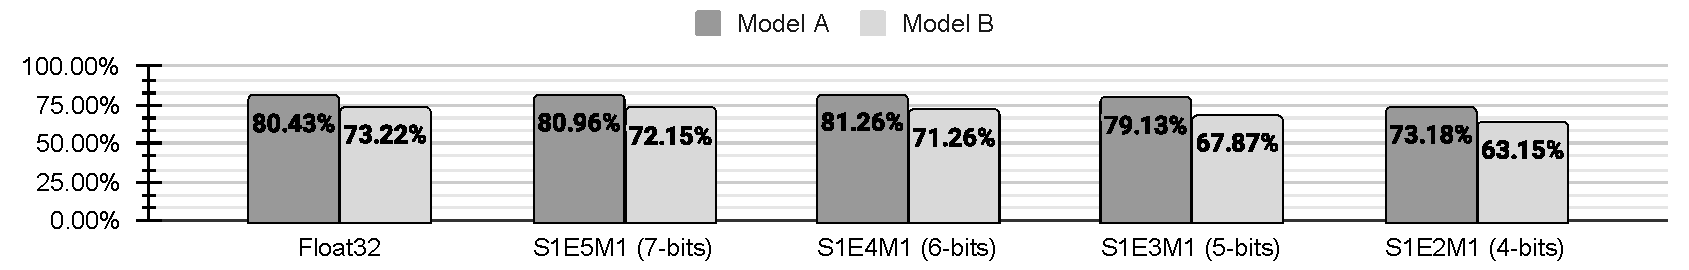
\includegraphics[width=0.5\textwidth]{../figures/all_models_accuracy.pdf}
	\caption{Accuracy performance using hybrid custom floating-point approximation with various formats. Samples: CIFAR-10 test dataset ($10,000$ images).}
	\label{fig:accuracy}
\end{figure}

\subsection{Resource utilization and power dissipation}
The resource utilization and power dissipation of the TP is listed in \tab{tab:resource}. The power dissipation of the Zynq device is presented in \fig{fig:power}. 


\subsection{Discussion}
\begin{enumerate}

	\item{\textbf{Energy consumption}}: The implementations with hybrid custom floating-point and logarithmic approximation are the most efficient with energy reduction of $954\times$ and $1,055\times$, respectively. \tab{tab:edp} presents the energy-delay product (EDP) and energy reduction in \emph{(4A) Conv} operator.
	
\begin{table}[!htp]\centering
	\caption{Energy consumption in tensor operation \emph{(4A) Conv}.}\label{tab:edp}
	\scriptsize
	\begin{tabular}{lrrrrr}\toprule
		\textbf{Engine} & \textbf{$t$ (ms)} &\textbf{Power (W)} &\textbf{EDP (J)} &\textbf{Reduction} \\\midrule
		CPU &5,564.79 &1.404 &7,812.97 &1.00 \\
		Hybrid custom floating-point &124.03 &0.066 &8.19 &\textbf{954.43} \\
		Hybrid logarithmic &123.32 &0.060 &7.40 &\textbf{1,055.92 }\\
		\bottomrule
	\end{tabular}
\end{table}
	
	\item{\textbf{Resource utilization}}: 
	
	\item{\textbf{Accuracy}}: The hybrid custom floating-point approximation presents the best trade off between QoR and energy-efficiency. The bfloat16 (brain floating-point with 16-bits) achieves a comparable QoR with floating-point 32-bits, see \fig{fig:accuracy}. To improve accuracy, the CNN models would require quantization aware training methods.
	
	\item{\textbf{Bottleneck}}: To increase performance, this implementation would require matching computational throughput with memory bandwidth using parallelization approaches.
\end{enumerate}